% Offizielle Beispieldatei für beamer-Vorlage aus tubslatex Version 0.3beta2
\documentclass[fleqn,11pt,aspectratio=43]{beamer}

\usepackage[ngerman]{babel}
\usepackage[utf8x]{inputenc}
\usepackage{graphicx}
\usepackage{listings}
\usepackage{color}
\usepackage{pxfonts}

\usetheme[%
  %cmyk,%<cmyk/rgbprint>,          Auswahl des Farbmodells
  orange,%<blue/orange/green/violet> Auswahl des Sekundärfarbklangs
  %dark,%<light,medium>        Auswahl der Helligkeit
  %colorhead,%    Farbig hinterlegte Kopfleiste
  %colorfoot,%    Farbig hinterlegt Fußleiste auf Titelseite
  colorblocks,%   Blöcke Farbig hinterlegen
  %nopagenum,%    Keine Seitennumer in Fußzeile
  %nodate,%       Kein Datum in Fußleiste
  %tocinheader,%   Inhaltsverzeichnis in Kopfleiste
  %tinytocinheader,% kleines Kopfleisten-Inhaltsverzeichnis
  %widetoc,%      breites Kopfleisten-Inhaltsverzeichnis
  %narrowtoc,%    schmales Kopfleisten-Inhaltsverzeichnis
  %nosubsectionsinheader,%  Keine subsections im Kopfleisten-Inhaltsverzeichnis
  %nologoinfoot,% Kein Logo im Fußbereich darstellen
  ]{tubs}

% Titelgrafik, automatisch beschnitten, Weitere Optionen: <scaled/cropx/cropy>
%\titlegraphic[scaled]{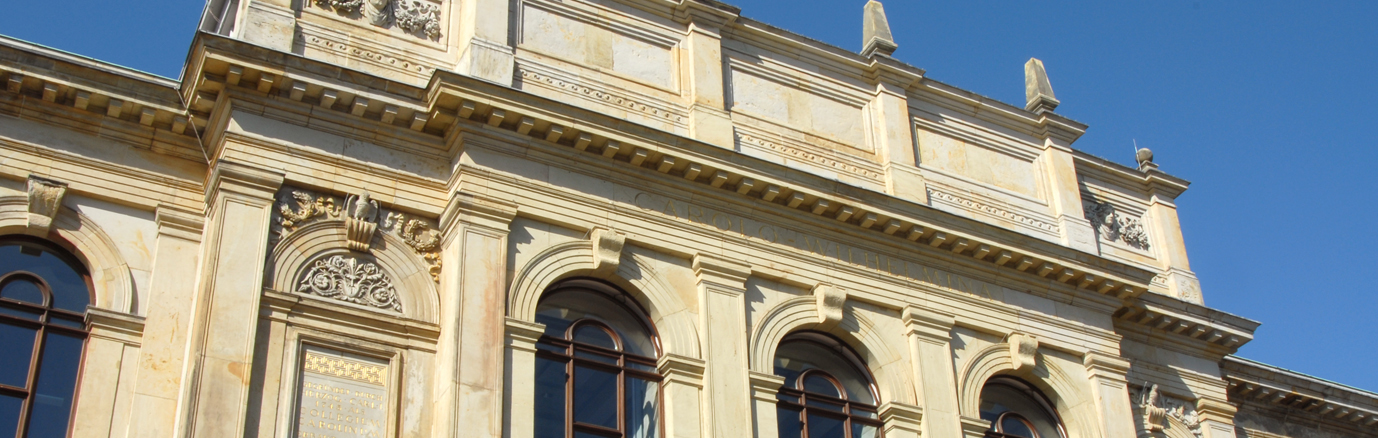
\includegraphics{img/titlepicture.jpg}}
\titlegraphic[cropy]{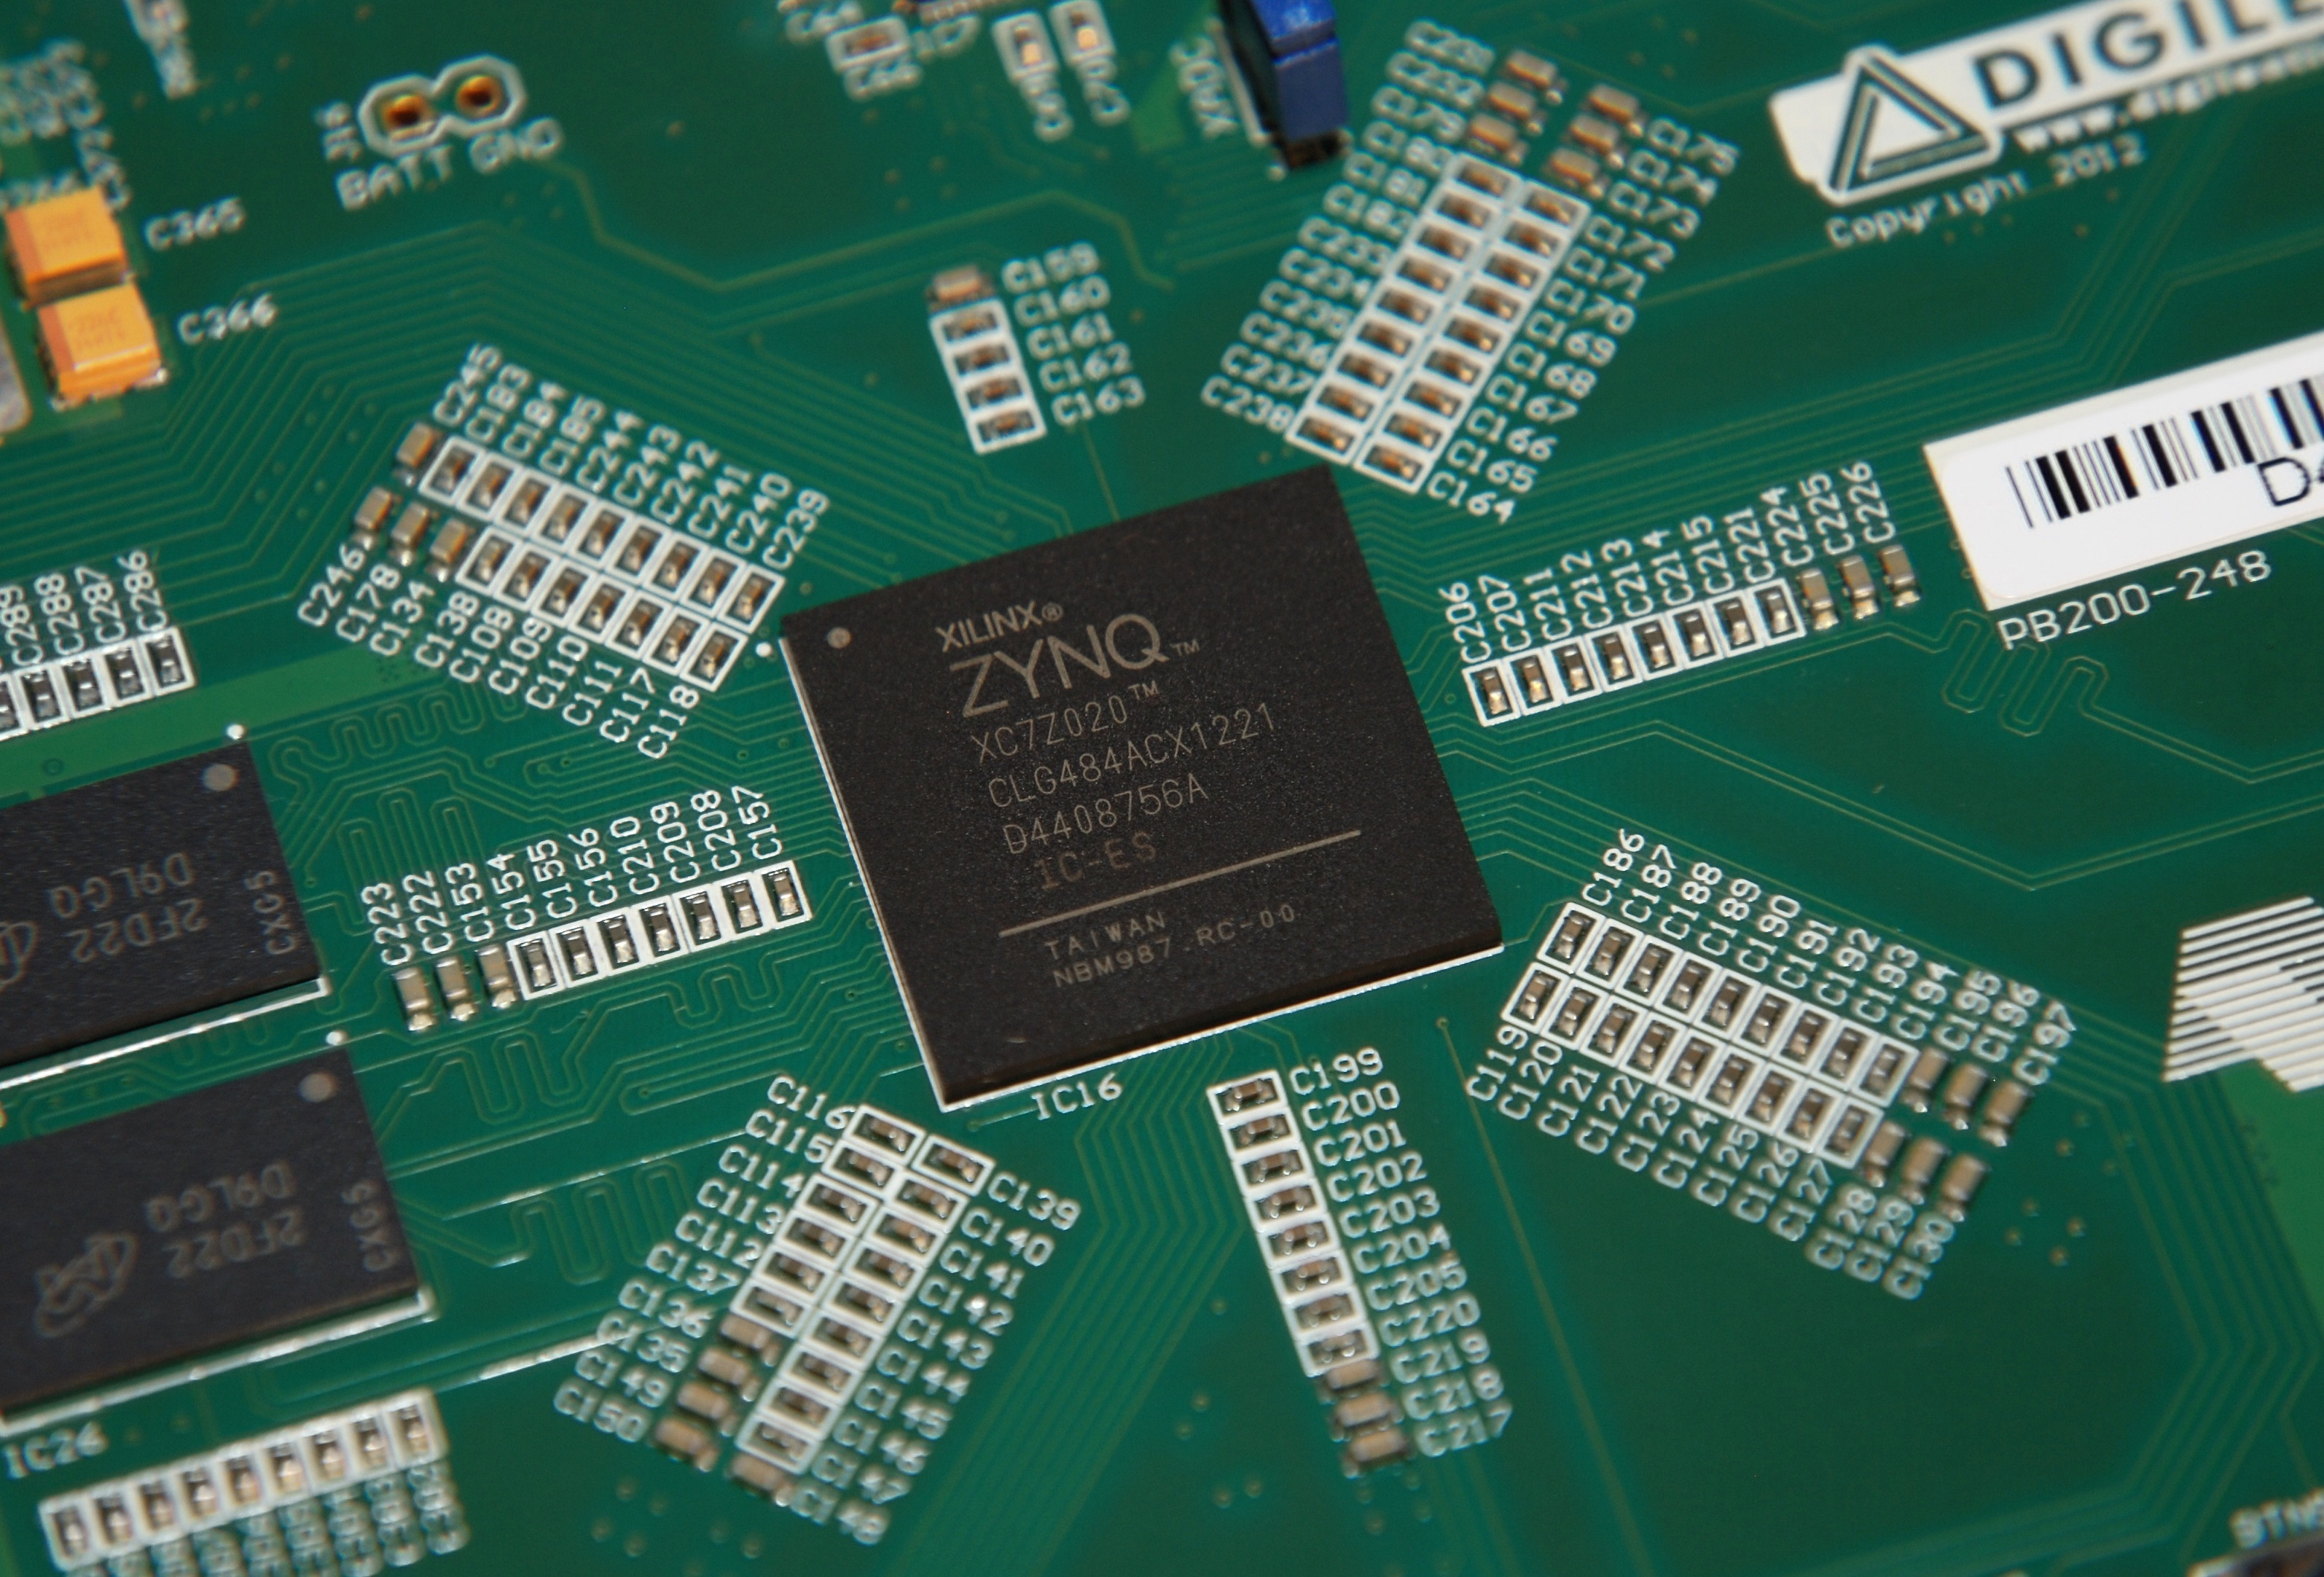
\includegraphics{img/zynq.jpg}}

% Logo, dass auf Titelseiten oben rechts und auf Inthaltsseiten unten rechts
% dargestellt wird. Es wird jeweils automatisch skliert
\logo{
\includegraphics{img/logo_mit_text.pdf}}

% settings for source code highlighting
\lstset{ %
  backgroundcolor=\color{white},         % choose the background color
  basicstyle=\ttfamily\footnotesize,     % size of fonts used for the code
  breaklines=true,                       % automatic line breaking only at whitespace
  captionpos=b,                          % sets the caption-position to bottom
  commentstyle=\color{tuGreenDark80},    % comment style
  escapeinside={\%*}{*)},                % if you want to add LaTeX within your code
  keywordstyle=\color{tuBlueMedium100}\bfseries, % keyword style
  stringstyle=\color{tuVioletMedium},    % string literal style
}

\defbeamertemplate*{section in toc}{my theme}
{\leavevmode\leftskip=0.5em\large{\usebeamercolor[fg]{titlelike}} 
\inserttocsection\par}

\defbeamertemplate*{subsection in toc}{my theme}
{\leavevmode\leftskip=2em\normalsize{\usebeamercolor[fg]{titlelike}} 
\inserttocsubsection\par}

\defbeamertemplate*{subsubsection in toc}{my theme}
{\leavevmode\leftskip=3.5em\normalsize\usebeamerfont{subsection in 
toc}\usebeamerfont{subsubsection in toc}\inserttocsubsubsection\par}

%\newif\iflattersubsect

\AtBeginSection[]{
  \begin{frame} 
  		\scriptsize
  		%\frametitle{\insertsectionhead}  
  		\frametitle{Überblick}  
  		%\begin{block}{\vspace*{-3ex}}
  			\tableofcontents[currentsection, hideallsubsections]
  		%end{block}
  		 
  		%\tableofcontents[currentsection, subsectionstyle=show/show/hide] 
  \end{frame}
%  \lattersubsectfalse
}

\AtBeginSubsection[]{
%\iflattersubsect
  \begin{frame} 
    	\scriptsize 
  		\frametitle{\insertsectionhead~- \insertsubsectionhead} 
  		%\begin{block}{\vspace*{-3ex}} 
  			\tableofcontents[ 
  		    	currentsubsection, 
  		    	sectionstyle=show/hide, 
  		    	subsectionstyle=show/shaded/hide
  		    	] 
  		%\end{block}
  		%\vspace{6cm}
  \end{frame}
%  \fi
%  \lattersubsecttrue
}

%\AtBeginSubsubsection[]{
%\iflattersubsect
%  \begin{frame} 
%    	\scriptsize 
%  		\frametitle{\insertsubsectionhead~- 
%  		\insertsubsubsectionhead} 
%  		%\begin{block}{\vspace*{-3ex}} 
%  			\tableofcontents[ 
%  		    	currentsubsection, 
%  		    	sectionstyle=show/hide, 
%  		    	subsectionstyle=show/shaded/shaded
%  		    	] 
%  		%\end{block}
%  		%\vspace{6cm}
%  \end{frame}
%  \fi
%  \lattersubsecttrue
%}

% Titelseite
\title{Seminar Technische Informatik}
\subtitle{Top 10 algorithms in data mining}
\author{Stephan Mielke}
\date{22.01.2015}

\begin{document}

\begin{frame}[plain]
\titlepage
\end{frame}

\begin{frame}{Inhalt}
\tableofcontents
\end{frame}

\section*{Einleitung~}

\begin{frame}[plain]{\insertsectionhead - Der Weltraum enendliche Weiten}

\begin{figure}
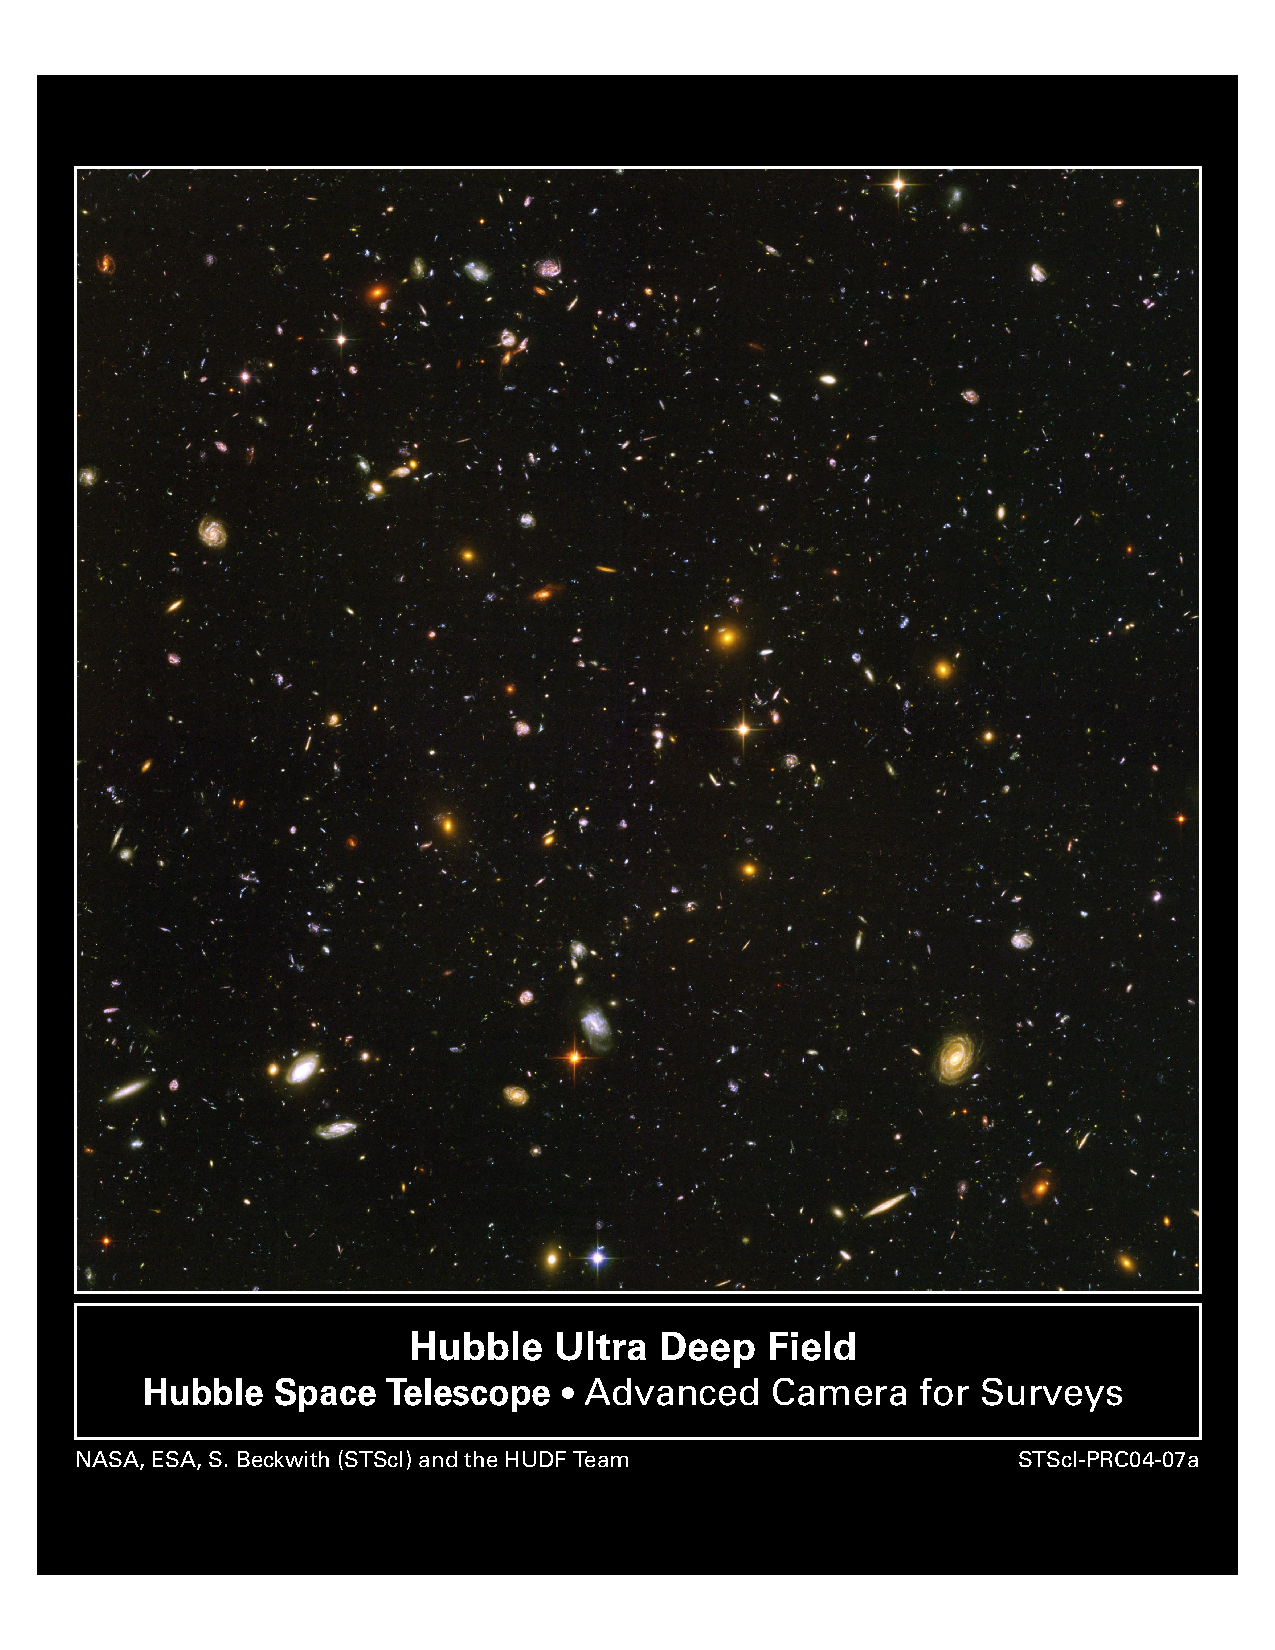
\includegraphics[scale=0.6,trim={40 400 40 80},clip]{hs-2004-07-a-pdf}
\caption{Hubble Ultra Deep Field\cite{HUDF}}
\label{fig:hs-2004-07-a-pdf}
\end{figure}

\end{frame}

\begin{frame}[plain]{\insertsectionhead - Einsatz von DM in der Astronomie}
\begin{itemize}
\item Teleskope erfassen pro Bild ca 10.000 Objekte 
\item Manuelle Klassifizierung unmöglich \cite{ester2000knowledge}
\item Benutzung von Klassifizierungsalgorithmen aus DM
\only<1>{\item Je Objekt 9 Attribute (8 Isophotenformen, Leuchtkraft)
\item Ausgabewert \glqq stellary\grqq 
\begin{itemize}
\item $0.0 - 0.1$ Galaxie
\item $0.9 - 1.0$ Stern
\end{itemize}} 
\end{itemize}
\pause
\begin{table}
\begin{tabular}{l|l}
Name & Erkennung\\ \hline
Random Forest & $82,89\%$ \\
Decision Tree & $80,68\%$ \\
Artificial Neural Network & $75.82\%$ \\
Support Vector Machines & $37,82\%$ \\
\end{tabular}
\caption{Erkennungsraten der Algorithmen Stern / Galaxie\cite{o2009star}}
\end{table}
\end{frame}



\section{Data Mining~}

\begin{frame}{\insertsectionhead -  Einleitung}

\end{frame}

\subsection{Klassifikation}
\subsubsection{Einleitung}
\subsubsection{Support vector machines}
\subsection{Clustering}
\subsubsection{Einleitung}
\subsubsection{k-means}
\subsection{Assoziation}
\subsubsection{Einleitung}
\subsubsection{Apriori}
\section{Top 10 algorithms in data mining}
\section{Neue Algorithmen}

\begin{frame}{Hier steht der Titel der Folie}
Wir beginnen mit einer Aufzählung
\begin{itemize}
  \item Aufzählzeichen werden als Quadrate dargestellt
  \begin{itemize}
    \item Unterpunkte ebenfalls
    \item Allerdings etwas kleiner
  \end{itemize}
\end{itemize}
\end{frame}

\section{Kapitel 2}


\begin{frame}{Itemize-Test}
  \begin{itemize}
    \item Lorem ipsum dolor sit amet, consetetur sadipscing elitr, sed diam
      nonumy eirmod tempor invidunt ut labore et dolore magna aliquyam
    \item At vero eos et accusam et justo duo dolores et ea rebum.
      \begin{itemize}
        \item Stet clita kasd gubergren, no sea takimata sanctus est Lorem ipsum
          dolor sit amet!
          \begin{itemize}
            \item Nam eget dui.
            \item Maecenas tempus, tellus eget condimentum rhoncus, sem quam
              semper libero, sit amet adipiscing sem neque sed ipsum.
          \end{itemize}
        \item Duis leo
      \end{itemize}
    \item Aliquam lorem ante, dapibus in, viverra quis, feugiat a, tellus. 
  \end{itemize}
\end{frame}


\subsection{Unterkapitel 1}


\begin{frame}{Mathe-Test}
  Gaußsche Summenformel:
  \[1 + 2 + 3 + 4 + \ldots + n = \sum_{k=1}^n k = \frac{n(n+1)}{2}\]
  Faltung:
  \[(f*g)(\xi) := \int_{\mathbb{R}^n} f(y)g(\xi-y)\mathrm{d}y\]
\end{frame}



\section{Ende}


\begin{frame}{Farbtest}
  \color{tuRed}
  Dies ist ein Text in tuRed.

  \color{tuSecondaryDark80}
  Dies ist ein Text in tuSecondaryDark80.

  \color{tuSecondaryLight}
  Dies ist ein Text in tuSecondaryLight.
\end{frame}


\begin{frame}{Verwendung von Spalten}
  \begin{columns}[onlytextwidth]
    \column{0.5\textwidth}
      Dies ist die erste Spalte.
      Die Angabe der Option \texttt{[onlytextwidth]}
      sorgt dafür, dass die Spaltenbreite korrekt eingehalten wird.
    \column{0.5\textwidth}
      Dies ist die zweite Spalte mit weiteren Informationen.
  \end{columns}
\end{frame}


\begin{frame}{Blöcke}
  \begin{block}{Diest ist ein Block}
    Lorem ipsum dolor sit amet, consetetur sadipscing elitr, sed diam
    nonumy eirmod tempor invidunt ut labore et dolore magna aliquyam
  \end{block}
  \begin{exampleblock}{Diest ist ein Example-Block}
    Lorem ipsum dolor sit amet, consetetur sadipscing elitr, sed diam
    nonumy eirmod tempor invidunt ut labore et dolore magna aliquyam
  \end{exampleblock}
  \begin{alertblock}{Diest ist ein Alert-Block}
    Lorem ipsum dolor sit amet, consetetur sadipscing elitr, sed diam
    nonumy eirmod tempor invidunt ut labore et dolore magna aliquyam
  \end{alertblock}
\end{frame}


\begin{frame}[fragile]{Quellcode}
Quellcode-Frames müssen immer die Option \texttt{[fragile]} tragen.
\begin{lstlisting}[language=c]
#include <iostream>

using namespace std;

// main function
int main() {
  cout << "Hello World!";
}
\end{lstlisting}
\end{frame}


\begin{frame}[highlight]{Wichtig}
Diese Folie ist wichtig!
\end{frame}

\begin{frame}
bla\cite{wu2008top}
\frametitle{Literatur}
\bibliographystyle{../IEEEtranBST/IEEEtran}
\bibliography{../lit}
\end{frame}

\end{document}
